
%----------------------------------------------------------------------------------------
%	PART
%----------------------------------------------------------------------------------------
%\part{실험}

%\chapterimage{chapter_head_1.pdf} % Chapter heading image
%\chapter{대기 관측}

\section{대기 관측 개관}\index{대기 관측 개관}

\subsection{필요성}\index{필요성}

대기 과학 이라는 학문은 정확한 일기예보를 하기 위한 노력에서 시작되었다고 볼 수 있다. 미래의 대기의 변화를 정학하게 예측한다는 것은 매우 어려운 일이지만 과거와 현재의 대기 상태를 토대로 그간의 경험 더해지면 아주 불가능한 일은 아니다. 정확한 일기 예보를 위해서는 대기의 열 역학적, 운동 역학적 특성을 명확하게 이해하고, 적절한 분석 기법, 모델 자료 등을 활용하여 미래의 대기 상태를 예측하는 능력이 필요하다. 

세계기상기구(WMO, World Meteorological Organization)는 보다 정확하고 표준화된 대기 관측에 대한 일반적인 지침을 제공하기 위해 ⌜대기 관측 측기와 방법에 관한 안내서(Guide to Meteorological Instruments and Methods of Observation)\을 발행하여 현업 기관에서 활용하도록 하고 있다. 이 문서는 WMO 산하에 있는 기상대에서 관측해야 하는 기상 요소들과 이에 필요한 측기들 그리고 이들을 운영 유지하는데 필요한 상세한 내용들을 포함하고 있다. 

\subsection{대표성}\index{대표성}

대기관측의 대표성이란 특정한 목적에 필요한 기상 변수들의 값이 얼마나 정확하게 설명되어 지는가를 의미한다. 따라서 대표성이란 어떤 특정한 관측 값을 의미하는 것이 아니라, 특정한 적용에 필요한 관측 주기와 대푯값 여부 등을 종합 판정해서 결정되어진다. 예를 들어, 종관 관측은 일반적으로 관측소 주변 100 km 지역까지를 대표할 수 있는 곳에서 이루어져야 하는 반면, 중규모나 국지규모 기상에 필요한 관측은 10 km 이하의 대표성을 가져도 된다.

대표성은 평균을 위한 시간적, 공간적 규모, 관측소 밀도, 기상 현상의 수평 규모 등에 따라서 결정되는데, 예를 들면 초단기 예보의 경우에는 시간적 공간적 규모가 작은 기상 현상들을 탐지해야 하기 때문에 그 만큼 좁은 지역에 조밀한 관측망을 구축해서 짧은 주기로 관측해야 빠르게 발달하고 소멸하는 기상 현상을 제대로 관측하고 예측할 수 있는 것이다. 

대표성을 확보할 수 있는 좋은 대기 관측은 관측 기술, 훈련, 장비와 지원 등이 충분히 이루어져야 가능하고, 적용되는 기상 업무에 따라 관측 주기도 다르게 구성되어야 한다.WMO 보고서와 다양한 연구 결과를 토대로 기상 현상의 수평 규모는 다음과 같이 구분할 수 있다.
\begin{itemize}
	\item 미규모(Microscale) : 100m 미만의 수평 규모를 가지며 주로 농업 기상학에 적용되고 주요한 관측 요소는 증발량이 있다.
	\item 국소(Toposcale) 혹은 국지규모(Local scale) : 100m에서 3km까지의 수평규모를 가지며, 대기 오염이나 토네이도 활동 등과 관련되어 있다.
	\item 중규모(Mesoscale) : 3km에서 100km의 수평규모를 가지며 뇌우, 해륙풍, 산악풍 등이 이에 해당한다.
	\item 대규모(Large scale) : 100km에서 3,000km의 수평 규모를 가지며 전선, 다양한 저기압, 구름 무리 등이 이 규모에 해당한다.
	\item 행성 규모(Planetary scale) : 3,000km 이상의 수평규모를 가지며, 대류권 상층의 장파가 이에 해당한다.
\end{itemize}

\begin{figure}
	\centering
	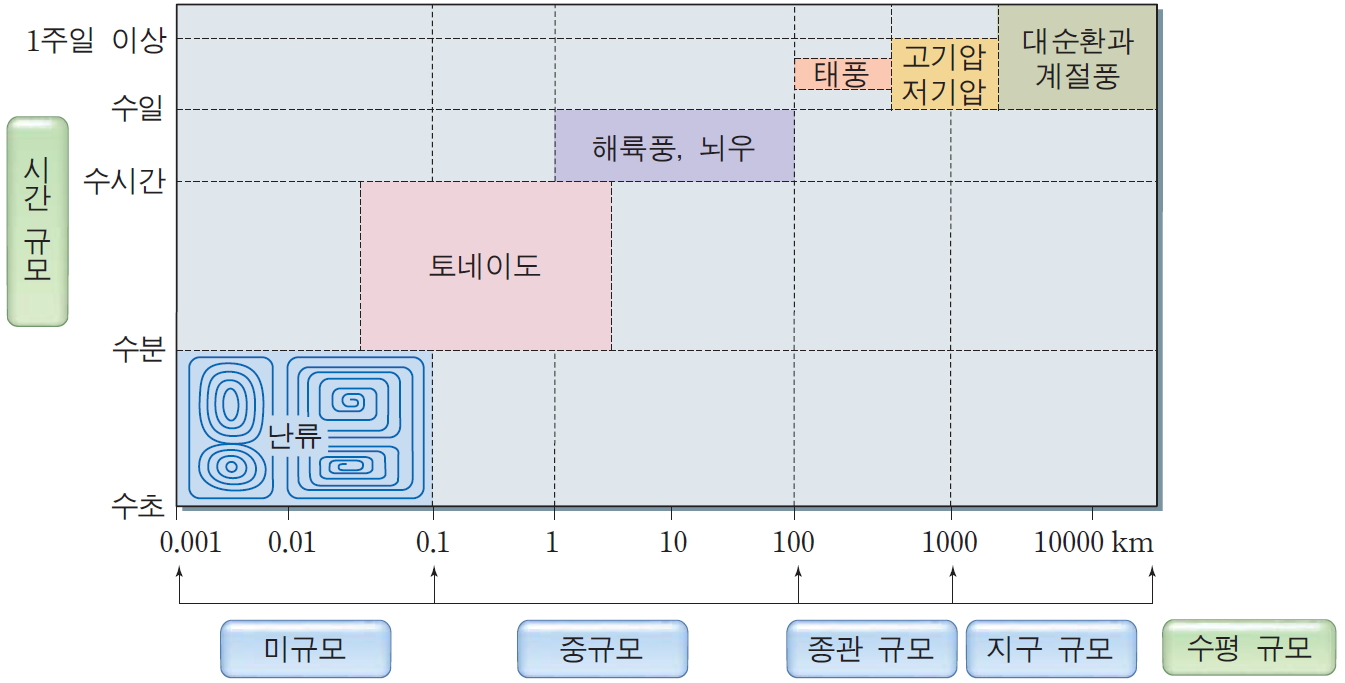
\includegraphics[width=0.9\linewidth]{21observing/images/C-E-o3O-F0-0301-00026-02}
	\caption{대기 순환의 규모}
	\label{fig:c-e-o3o-f0-0301-00026-02}
\end{figure}


\subsection{대기 관측 체계}\index{대기 관측 체계}

정확한 대기 관측을 위해서는 다양한 센서들을 구비한 적절한 관측 기구와 원격 탐사 체계가 필요하다. WMO는 전구 규모, 지역 규모, 국가 규모의 관측을 위해서 필요한 대기 관측  체계에 관한 지침을 제공하고 있다. 전구 규모의 관측에 부합하기 위해서는 지상 기반의 하부 체계와 위성 기반의 하부 체계가 통합된 형태의 대기 관측 체계를 구축하여야 한다. 지상 기반 하부 체계는 지상 종관 기상대, 고층 관측, 기후 관측 등을 포함하며, 위성 기반 하부 체계는 기상 위성과 자료 송수신 체계를 포함한다. 지역 규모와 국가 규모의 관측은 주로 지상 기반의 관측 체계로 구성되어진다. 

\subsection{지상 관측 기상 요소들}\index{지상 관측 기상 요소들}

기상 관측의 목적과 체계에 따라 다양한 요구 조건들이 주어지지만 WMO에서 권고하는 대기 관측 요소들은 다음과 같다.

\begin{itemize}
	\item 현재 기상
	\item 과거 기상
	\item 풍향과 풍속
	\item 운량
	\item 운형
	\item 운저 고도
	\item 시정
	\item 온도
	\item 상대습도
	\item 기압
	\item 강수량
	\item 적설
	\item 일사/태양복사량
	\item 토양온도
	\item 증발량
\end{itemize}

\subsection{자동 기상 관측 시스템 (AWS: Autometic Weather System)}\index{자동 기상 관측 시스템 (AWS: Autometic Weather System)}

정보 통신 기술의 발달과 함께 다기능 기상 관측 센서를 가진 자동 기상 관측 시스템 (AWS: Autometic Weather System) 을 네트 워크로 연결하는 기상 관측 체계가 대세를 이루고 있다. 종관, 기후, 항공 기상 분야에서 필요한 대부분의 기상 요소들은 자동 관측 장비를 통해서 관측할 수 있다. AWS의 발전과 함께 전체 관측소에서 순수한 자동기상 관측소가 차지하는 비율이 관측자에 의한 관측소에 비해서는 여전히 작지만 꾸준하게 증가하고 있는 추세에 있다. 다만, AWS로 관측된 값들이 대표성과 유용성을 확보하기 위해서는 적절한 관측 지점 선정, 주기 적인 센서 교환과 정비 활동 등이 반드시 필요하다.

\begin{figure}[h]
	\centering
	\begin{minipage}{.65\textwidth}
		\centering	
		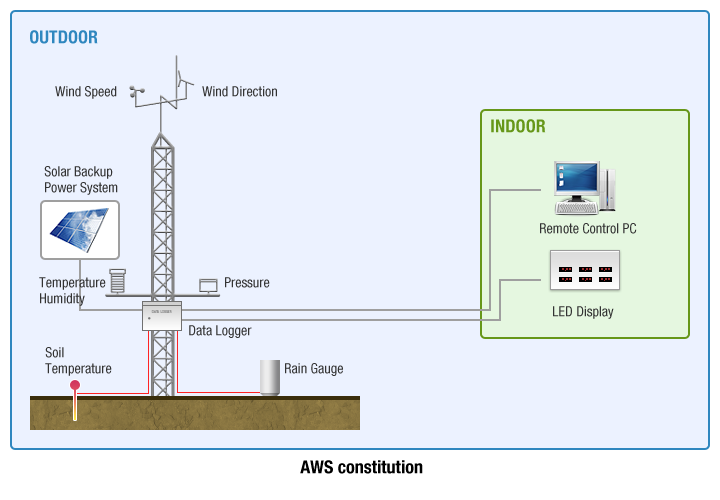
\includegraphics[width=0.95\linewidth]{21observing/images/aws1}
	\end{minipage}
	\begin{minipage}{.33\textwidth}
		\centering
		\includegraphics[width=0.95\linewidth]{21observing/images/20160421_184928}
	\end{minipage}
	\caption{AWS 개요와 실물}
	\label{fig:aws}
\end{figure}


\subsection{관측자의 중요성}\index{관측자의 중요성}

대기 관측 요소들 중에서 운형을 제외한 나머지 요소들을 자동으로 관측할 수 있는 센서들은 이미 개발되어 활용되고 있다. 그러나 센서와 정보통신 기술력을 모두 통합한다고 하더라도 현재 기상, 과거 기상, 운량과 운고, 적설과 같은 기상 요소들을 완벽하게 망라할 수 있는 대기 관측 체계는 존재하지 않기 때문에 결국 사람에 의한 관측은 기술 발전과 무관하게 매우 중요하고 가장 정확한 방법으로 남아있으며 다음과 같은 관측자의 역할은 여전히 중요하다.

\begin{itemize}
	\item 종관/기후 관측에 있어서 적절한 관측 도구의 도움을 받아 불확실성을 제거하고 관측 값들이 대표성을 가질 수 있도록 관측이 이루어져야 한다.
	\item 관측 기구들의 상태를 양호하게 유지하고, 관측자료들을 관리하는 등 관측소가 좋은 상태를 유지할 수 있도록 한다.
	\item 자동 코딩이나 통신망이 갖추어지지 않은 지역에서의 긴급한 관측과 전송이 필요한 경우가 많다.
	\item 자동화되어 있지 않은 관측소의 주간/월간 단위 기후학적 자료 정리와 기록이 필요하다.
	\item 자동 관측 체계는 다양한 이유로 인해서 필요한 관측 요소를 관측하지 못하거나 관측 체계 전체가 고장날 수 있기 때문에 보조 혹은 백업 관측이 반드시 필요하다.
	\item 관측자는 다양한 전문적인 관측 요구에 부응할 수 있다. 따라서 관측자는 필요로한 표준화된 관측을 할 수 있도록 훈련되어지고 검증된 기상 기관에서 자격을 부여받은 사람이어야 한다. 
	\item 관측자는 관측 기구의 사용법에 대해서 이해하고 있어야 하며 관측 기구를 통해 필요한 관측 요소들을 적절하게 관측할 수 있도록 훈련되어야 한다.
\end{itemize}
	
\subsection{관측소의 선정}\index{관측소의 선정}
관측소 선정의 가장 큰 기준은 관측값이 대표성을 가지도록 하는 것이다. 종관 관측망에 포함되어 있는 관측소는 종관 규모 요구도에 부합하도록 선정되어야 하며, 항공기상을 지원하는 관측소는 국지(공항)에 특화된 특수한 조건들에 부합하도록 위치가 선정되어야 대표성을 확보할 수 있다. 관측소의 설치와 구성에 관한 내용은 WMO 지침에 상세하게 규정되어 있는데
지역 규모 혹은 국가 규모 관측망에 포함되는 전형적인 종관 규모 관측소는 다음과 같은 선정 기준이 제시되고 있다.

\begin{itemize}
	\item 외부에 설치되는 관측기구들은 지상으로부터 일정한 높이에 설치되어야 하며, 전체 관측 야장은 25 m × 25 m 보다 큰 규모를 권장하지만 부득이한 경우에는 최소한 10 m × 7 m 까지 축소할 수 있다. 
	\item 관측소의 바닥은 짧은 잔디나 주변 지표면 특성을 대표할 수 있는 토양으로 구성되어 있어야 하고, 관측 장비가 설치된 구역은 바람이 통하는 울타리를 설치하여 비인가 인원의 출입을 막아야 한다. 
	\item 관측 구역 내에 2 m × 2 m 의 맨 땅을 만들어 지표면 상태와 토양 온도를 관측할 수 있도록 하여야 하는데 토양 온도는 20 cm 미만의 깊이에서 관측하여야 한다.
	\item 관측소 주변에는 가파른 지형이 없어야 하며 우묵한 곳이나 공동 구역에 설치하지 않아야 하는데 이러한 규칙이 지켜지지 않으면 관측소는 대표성을 확보할 수 없다.
	\item 관측소는 나무, 건물, 벽, 장애물 등으로부터 충분히 멀리 떨어져 있어야 한다. 우량계는 울타리를 포함한 우량계 주변의 장애물이 우량계 높이보다 2배 이상 떨어져 있도록 설치되어야 하는데 가능하면 4배 이상 떨어져 있는 것이 좋다.
	\item 일사/복사 측정기, 우량계, 풍향풍속계는 동일한 장소에 서로 충분히 노출되도록 설치되어야 한다.
	\item 풍향풍속계는 장애물에 의해서 왜곡이 심할 가능성이 높기 때문에 어떠한 경우에도 장애물로 둘러싸여 있어서는 안 되며, 항상 사방이 열린 곳에 설치되어야 한다.
	\item 대부분의 측기는 사방이 완전히 열려있는 것이 유리하지만, 우량계의 경우에는 강한 바람에 의해서 강수량이 왜곡될 수 있기 때문에 바람의 영향을 적게 받도록 어느 정도의 엄폐 장치가 필요하다.
	\item 일사나 복사량 관측에 있어서 측기가 나무나 건물 등과 같은 장애물로 가려져 수평적인 관측이 크게 제한을 받은 경우 충분한 관측이 가능하도록 대체 장소를 찾아야 한다.
	\item 구름이나 시정을 관측하는 지점은 가능한 사방의 관측이 가능한 열린 곳이어서 주변 지역과 하늘을 충분히 관측할 수 있는 곳이어야 한다.
	\item 해안에 설치되는 관측소는 바다가 보이는 방향으로 설치하는 것이 좋다. 그러나 관측소가 너무 해안에서 가깝거나 절벽에 위치하는 경우에는 장애물에 의한 난류 발생으로 바람과 강수량 관측에 영향을 미칠 수 있다.
	\item 구름과 시정을 야간에 관측할 경우에는 외부 불빛으로부터 영향을 받지 않는 지역에서 실시하여야 한다.
\end{itemize}


\subsection{관측소 좌표}\index{관측소 좌표}
<<<<<<< HEAD
관측소의 위치는 세계 측지 체계 1984 (WGS-84, World Geodetic System 1984) 와 지구 측지 모델 1996 (EGM96,Earth Gravitational Model 1996) 의 기준에 따라 정확하게 좌표로 지정되어야 한다. 관측소 좌표는 위도와 경도값은 0.0001 $\rm ^{\circ}$ 까지 상세하게 보고되어야 하며, 관측소의 높이도 해발 고도로 미터 (m) 단위로 보고되어야 한다.

\subsection{측기의 바람직한 특성들}\index{측기의 바람직한 특성들}

측기가 가지는 불확실성, 신뢰성, 안정성은 측기가 일단 설치되면 오랜 기간 동안 운영 유지되어야 한다는 점에서 가장 중요한 고려 요소가 된다. 측기를 운영하는 초기에 불확실성 정도에 대한 정확한 정보를 가지고 있는 것이 측기를 운영하는 전 과정 동안 발생할 수 있는 문제점을 사전에 인지하는데 유리하다.

일반적으로 측기의 초기 보정은 이상적인 값과 관측값 사이의 편차를 줄이는 과정에서 중요한 의미를 가지며, 측기들은 운영하는 동안 지속적인 정비 활동과 검증 및 보정 작업이 필요하며, 보정 작업이 필요한 시기와 이상 징후에 대한 정확한 정보가 관측자에게 주어져야 한다.

디자인의 단순함과 내구성은 장비설치, 운영 및 유지에 있어서 중요한 고려 요소가 된다. 왜냐하면 보통 기상 측기는 연중 무중단 운영되며 전문적인 수리가 가능한 지역에서 멀리 떨어진 곳에 설치 운영되는 경우가 많기 때문이다.

대기관측에 이용되는 측기의 중요한 요구 조건들은 다음과 같다.

\begin{itemize}
	\item 특정한 변수들에 대해서 어느 정도의 불확실성을 가지는지 명확해야 함
	\item 신뢰성과 안정성
=======
관측소의 위치는 세계측지체계 1984 (WGS-84) 와 지구측지 모델 1996 (EGM96) 의 기준에 따라 정확하게 좌표로 지정되어야 한다. 관측소 좌표는 위도와 경도값은 0.0001 $\rm ^{\circ}$ 까지 상세하게 보고되어야 하며, 관측소의 높이도 해발 고도로 미터(m) 단위로 보고되어야 한다. 관측소의 좌표는 실제 관측이 이루어지는 지점을 의미하며 같은 이름의 도시나 마을, 공항의 위치를 의미하는 것이 아니다. 종관 관측이 이루어지는 관측소의 높이는 일반적으로 해발고도로 우량계가 서 있는 지역의 높이를 의미한다. 우량계가 없는 관측소는 백엽상의 높이를 의미한다. 공항과 같이 관측소 기압이 매우 중요한 지역의 경우에는 관측소의 높이는 실제 기압 관측이 이루어지는 고도에 맞추는 것이 좋다.

\subsection{측기의 특성과 균질성의 변화}\index{측기의 특성과 균질성의 변화}
관측소의 특성은 나무의 성장이나 주변 건물의 신축 등과 같은 요소들에 의해서 시간에 따라 계속해서 변화할 수 있기 때문에 관측소는 이러한 환경의 변화가 최소화될 수 있는 지역에 설치되는 것이 좋다. 가능하면 관측소 주변 환경의 변화를 지속적으로 기록하여 필요한 경우에는 적절한 대체 장소를 선정하는데 활용하여야 한다. 측기의 교체나 위치를 변경할 경우에는 그 영향이 최소화될 수 있도록 방법을 강구하여야 한다. 비록 새로운 장비의 물리적인 특성은 잘 알려져 있다고 하더라도 현업에 활용하기 위해서는 반드시 그 지역의 기후학적 특성에 맞추어 적절하게 보정되어야 한다.

WMO는 새로운 측기를 설치하여 운영하는 경우에 이전 장비를 철수하기 전에 최소한 1년 정도의 비교 관측을 통해서 안정성을 확보하도록 권고하고 있다. 이러한 기준은 관측 장소를 옮겼을 경우에도 동일하게 적용된다. 
대기관측에 이용되는 측기의 중요한 요구 조건들은 다음과 같다.

\begin{itemize}
	\item 불확실성. 특정한 변수들에 대해서 어느 정도의 불확실성을 가지는지 명확해야 한다.
	\item  신뢰성과 안정성
>>>>>>> baf41d259c4748754a83ad0ee0d9825a7efd766b
	\item 작동의 편의성, 원활한 보정과 정비
	\item 디자인의 단순함
	\item 내구성
	\item 측기, 소모품, 부속품의 합리적인 유지비용
\end{itemize}

<<<<<<< HEAD
\subsection{측기의 균질성의 변화}\index{측기의 균질성의 변화}
관측소 주변은 나무의 성장이나 주변 건물의 신축 등과 같은 요소들에 의한 변화가 최소화 되어야 한다. 가능하면 관측소 주변 환경의 변화를 지속적으로 기록하여 필요한 경우에는 적절한 대체 장소를 선정하는데 활용하여야 한다. 

측기의 교체나 위치를 변경할 경우에는 그 영향이 최소화될 수 있도록 방법을 강구하여야 하며, 물리적인 특성이 잘 알려진 새로운 장비를 활용할 때에도 반드시 그 지역의 기후학적 특성에 맞추어 적절하게 보정되어야 한다. WMO는 새로운 측기를 설치하여 운영하는 경우에 이전 장비를 철수하기 전에 최소한 1년 정도의 비교 관측을 통해서 안정성을 확보하도록 권고하고 있다. 이러한 기준은 관측 장소를 옮겼을 경우에도 동일하게 적용된다. 
=======
\subsection{측기의 바람직한 특성들}\index{측기의 바람직한 특성들}

측기가 가지는 불확실성, 신뢰성과 안정성은 측기가 일단 설치되면 오랜 기간 동안 운영 유지되어야 한다는 점에서 가장 중요한 고려 요소가 된다. 측기를 운영하는 초기에 불확실성 정도에 대한 정확한 정보를 가
지고 있는 것이 측기를 운영하는 전 과정 동안 발생할 수 있는 문제점을 사전에 인지하는데 유리하다.
일반적으로 측기의 초기 보정은 이상적인 값과 관측값 사이의 편차를 줄이는 과정에서 중요한 의미를 가지며, 측기들은 운영하는 동안 지속적인 정비 활동과 검증 및 보정 작업이 필요하며, 보정 작업이 필요한 시기와 이상 징후에 대한 정확한 정보가 관측자에게 주어져야 한다.
디자인의 단순함과 내구성은 장비설치, 운영 및 유지에 있어서 중요한 고려 요소가 된다. 왜냐하면 보통 기상 측기는 연중 무중단 운영되며 전문적인 수리가 가능한 지역에서 멀리 떨어진 곳에 설치 운영되는 경우가 많기 때문이다.
>>>>>>> baf41d259c4748754a83ad0ee0d9825a7efd766b

\section{관측 값}\index{관측 값}

\subsection{단위}\index{단위}

관측을 실시하는 목적은 관측 지점의 대기의 상태에 대하여 정량화된 값을 제공하는데 있다. 대기 과학적 측면에서는 측정 값은 풍속 10 m/s, 기압 1013 hPa 등으로 대부분의 경우 앞 쪽에 관측값을 표시하고 바로 이어서 단위를 표시한다.
기상정보는 전 세계에 통용되어야 하기 때문에 대기관측에서 사용되는 단위들은 국제 표준 단위(SI)를 사용할 것을 권장하지만 대기과학에서만 적용되는 단위들을 사용하기도 한다. 그리고 기상 변수들에는 그것이 무엇을 의미하는지를 기호로 나타내기도 한다. 예를 들어 대기압은 ‘p’를 사용하여 기압임을 표시한다. 다음은 대기관측에서 사용되는 단위들이다.
<<<<<<< HEAD

\begin{itemize}
	\item 대기압(p) : 헥토파스칼 (hPa)
	\item 온도(t) : 섭씨($\rm ^{\circ}C$), 캘빈 온도(T) : 캘빈(K)
	\item 풍속 : 초속 ($\rm m~s^{-1}$)
	\item 풍향 : 불어 오는 방향을 10도($\rm ^{\circ}$) 단위로 표시. 36은 북풍, 09는 동풍을 의미
	\item 상대습도(U) : 퍼센트(\%)
	\item 강수량 : 밀리미터 (mm) 혹은 단위 면적당 무게($\rm {kg~m^{-2}}$)
	\item 강수 강도(Ri) : 단위 시간당 밀리미터 ($\rm {mm~h^{-1}}$)
	\item 강설량 : 단위 면적당 무게($\rm {kgf~m^{-2}}$)
	\item 증발량 : 밀리미터 (mm)
	\item 시정 : 미터 (m)
 	\item 조도 : 단위 면적 당 와트($\rm {W~m^{-2}}$)
	\item 복사량 : 단위 면적 당 주울($\rm {J~m^{-2}}$)
	\item 일조 시간 : 시간 (h)
	\item 운고 : 미터 (m)
	\item 운량 : 옥타 (Oktas)
\end{itemize}
=======
>>>>>>> baf41d259c4748754a83ad0ee0d9825a7efd766b

\begin{itemize}
	\item 대기압(p), 단위 : 헥토파스칼 (hPa)
	\item 온도(t), 단위 : 섭씨($\rm ^{\circ}C$) 혹은 캘빈 온도(T), 단위 : 캘빈(K)
	\item 지상풍과 상층풍 풍속, 단위 : 초속 ($\rm m~s{-1}$)
	\item 풍향, 불어 오는 방향을 표시. 36은 북풍, 09는 동풍을 의미, 단위 : 도($\rm ^{\circ}$)
	\item 상대습도(U), 단위 : 퍼센트(\%)
	\item 강수량, 단위 : 밀리미터 (mm) 혹은 단위 면적당 무게($\rm {kg~m^{-2}}$)
	\item 강수 강도(Ri), 단위 : 단위 시간당 밀리미터 혹은 단위 면적당, 단위 시간당 무게 ($\rm {kg~m^{-3}~h{-1}}$)
	\item 강설량, 단위 : 단위 면적당 무게($\rm {kg~m^{-2}}$)
	\item 증발량, 단위 : 밀리미터(mm)
	\item 시정, 단위 : 미터(m)
	\item 조도, 단위 : 단위 면적 당 와트($\rm {W~m^{-2}$)
	\item 복사량, 단위 : 단위 면적 당 주울($\rm {J~m^{-2}}$)
	\item 일사 시간, 단위 : 시간(h)
\end{itemize}
\subsection{상수}\index{상수}
<<<<<<< HEAD
=======
다음은 대기관측에서 사용되는 상수들이다.
\begin{itemize}
	\item 어는 점($T_0$)에서의 절대 온도 $\rm {= 273.15~K~(~=~0.00 ^{\circ}C)}$
	\item 물의 삼상 변화 절대 온도 $\rm {= 273.16~K~(~=~0.01 ^{\circ}C)}$
	\item 표준 중력가속도$\rm {(g_n)~=~9.80665(m~s^{-2})$
	\item 0$\rm ^{\circ}C$에서의 수은 농도 $\rm {= 1.35951~×~10^4~(kg~m^{-3})$
	\item 운고, 단위 : 미터 (m)
	\item 운량, 단위 : 옥타 (Oktas)
	\item 상층 지위 고도, 단위 : 지위고도 (gpm)

\end{itemize}

\subsection{관측 자료 조건}\index{관측 자료 조건}
\subsubsection{기압}\index{기압}

주어진 표면에서의 대기의 압력(이하 기압)은 표면 상공의 공기의 무게에 의해서 단위 면적당 가해지는 힘으로 정의된다. 따라서 기압은 지표면에서 대기의 상단까지 뻗어 있는 공기 기둥의 무게와 같다. 실제 기압과 별도로
기압의 변화 경향도 잘 측정되어야 한다. 기압 변화 경향은 관측 시간 바로 이전 3 시간 동안의 기압 변화량을 의미한다. 기압 변화 경향은 기압 자체의 변화와 기압 변화 특성으로 나누어질 수 있다. 기압 자체의 변화는 문자 그대로 일정한 시간 간격을 두고 관측된 처음과 끝의 기압 값의 차이를 의미한다. 기압변화 특성은 일정한 시간 동안 기압이 어떻게 변화해 왔는지에 대한 표시를 의미한다. 예를 들어 기압이 지난 3시간 동안 하강한 후에 상승했는지, 서서히 상승 하다가 급하게 상승 했는지가 기압 변화 특성이 된다.

압력의 기본 단위는 파스칼 (Pa) 혹은 ($\rm {N~m^{-2})$이지만 기압값은 앞에 100을 의미하는 헥토 (hecto)를 붙여서 헥토파스칼(hPa)을 사용한다. 기존에 기압의 단위로 많이 사용되었던 밀리바(mb)와 hPa은 같은 값이며, 몇몇 기압계들은 그 눈금 단위를 밀리바나 수은주 높이(mmHg)로 표시할 수 있는데, 표준 대기 상태에서 기압이 1013.250 일 때 수은주는 760 mmHg 의 높이를 가지게 되므로 기압의 단위는 다음과 같이 변환할 수 있다.
	
1 hPa = 0.750062(mmHg), 1(mmHg) = 1.333224 hPa

일반적으로 공학에서 사용되는 밀리미터와 인치 사이에는 1 in = 25.4 mm의 관계식을 가지게 되므로 다음과 같이 변환할 수 있다.

1 hPa = 0.029530 (inHg), 1 (inHg) = 33.8639 hPa, 1 (mmHg) = 0.03937008 (inHg)

분석된 기압장은 대기 과학적인 측면에서 볼 때 가장 필요한 요소이다. 기압장은 현재의 대기의 상태를 분석을 통해서 예측으로 이어지는 일련의 기상 업무에서 가장 기본적인 요소이므로 반드시 관측이 이루어져야 한다. 기압 관측은 기술이 허용하는 한 정확하여야 하며, 관측 도구들은 균질한 관측이 보장될 수 있도록 철저하게 보정이 이루어진 후에 관측에 투입되어야 한다.
대기관측에서 사용되는 수은 기압계의 눈금은 바로 실제 기압을 표준 단위로 읽을 수 있도록 눈금으로 표시되어야 한다. 모든 측기들은 표준 기온0$\rm ^{\circ}C$, 중력 가속도 9.80665($\rm m~s{-2}$) 에서 정해진 값이 표현되도록 유지되어야 한다. 기압계에는 보통 1개 이상의 눈금이 표시되어 있는데, 과 혹은
과 in 가 동시에 표시되어 있고 표준 대기 상태에서 기압계는 정확하게 보정되어 사용되어야 한다. 그런데 대기관측에서 항공기상과 같은 특별한 목적이 있는 경우를 제외하고는 기압값을 보고할 때는 단위로 표시
하여야 한다.

기압관측은 다음과 같은 요구 조건들을 만족하여야 한다.
관측 범위 : 관측소 기압과 해면기압 모두 500 ~ 1080
불확실성(오차) : 0.1 이하
보고 단위 : 0.1
관측 센서 지속 시간 : 20초
자료 표출 주기 : 1분 이하
위에서 언급된 요구조건들을 만족시키기 위해서는 새로운 기압관측 측기
들을 설치할 경우 장비를 현장에 설치하기 이전에 적절한 장비가 구비되고
엄격한 환경에서 검증을 통과한 측기로 보증을 받은 제품을 사용하는 것이
우선되어야 한다. 기압계들은 단독으로 설치 운영되는 경우보다 복합 기상
관측 장비의 일부로 구성되어 있거나, 네트워크로 연결되어 사용될 가능성
이 높기 때문에 장비를 현장에 설치할 때는 사전에 이러한 조건들을 만족
하는지를 강제적으로 확인할 필요가 있다. 또한 장비를 설치 운영하는 동안
지속적인 유지 보수와 보정 작업을 통해서 위의 요구 조건들에 계속해서
부합되도록 관리되어야 한다.

\subsubsection{기온}\index{기온}
WMO는 온도를 물체(고체, 액체, 기체) 속의 분자들의 평균 무작위 운동으
로 특징 지워지는 물리량으로 정의하고 있다. 온도는 두 개의 물체가 어떤
형태로 접촉하여 동등한 온도로 가고자 하는 행위로 특징 지워진다. 따라서
온도는 물체의 열역학적 상태와 두 물체 사이에서의 순수한 열 이동 방향
을 결정하는 물리량으로 표현된다. 두 개의 물체 사이에서 열을 잃는 물체
를 높은 온도라고 표현한다. 그러나 물체의 상태와 관련해서 온도의 물리량
을 정의하는 것은 매우 어려운 일이다. 국제적으로 인정받고 있는 온도 척
도는 물의 삼중점과 어는점을 이용하는 방법이다. 최근 국제적인 공인 온도
척도는 국제온도척도 1990(ITS-90)이다. 대기과학적 온도 범위(-0℃ ~
+60℃)에 대해서 이 온도 척도는 백금의 전기 저항과 273.16K로 정의되
어지는 물의 삼중점과의 선형 관계식을 기초로 하여 만들어진 것이다.
대기관측에 있어서 온도는 다양한 매체를 상대로 측정한다. 가장 일반적인
측정 변수는 다양한 고도에 대한 기온이고, 다른 것들로는 지표면, 토양, 잔

디, 해수면 온도 등이다. WMO는 기온을 “태양의 직접 복사로부터 차폐된
곳의 공기 중에 노출된 온도계가 가리키는 온도”로 정의하고 있다. 비록 이
정의가 그 자체의 열역학적 물리량으로 정의되는 것은 아니지만 광범위 하
게 적용되고 있다.

켈빈 단위(K )를 가지는 열역학적 온도(T ) 혹은 켈빈 온도가 기본 온도가
된다. 켈빈은 물의 삼중점으로부터 열역학적 온도가 1/273.15 씩 변화하는
단위를 말한다. 열역학적 온도에 대응하여 대기과학에서 주로 사용하는 섭
씨() 단위로 나타내는 온도(t )는 아래의 방정식 (1.1)과 같이 정의된다.

t/℃ = T/K - 273.15

섭씨(℃) 1도의 온도 차이는 켈빈 온도(K) 1도 단위와 같다. K 단위는 도(°)
와 함께 표시하지 않는다는 점에 주의해야 한다. 열역학적 온도 척도에 있
어서 온도의 측정은 절대온도 0도(0K)와의 차이로 표현되는데, 절대 온도
0K에서 모든 물질의 분자들은 운동 에너지를 갖지 않는다.
ITS-90에서 사용되는 온도 척도는 몇 가지 물질들의 재생 가능한 평형 상
태에서의 값을 기준으로 하며, 온도 관측 표준 장비들은 이 온도에 맞춰 보
정된다. 국제표준온도 척도는 각 물질들의 이상적인 열역학적 온도와 실제
온도와의 차이를 측정하여 관측기구의 불확실성 정도를 결정한다.
>>>>>>> baf41d259c4748754a83ad0ee0d9825a7efd766b

다음은 대기 관측에서 사용되는 상수들이다.

\begin{itemize}
	\item 어는 점($T_0$) : $\rm {= 273.15~K~(~=~0.00 ^{\circ}C)}$
	\item 물의 삼중점 : $\rm {= 273.16~K~(~=~0.01 ^{\circ}C)}$
	\item 표준 중력가속도: $\rm {(g_n)~=~9.80665(m~s^{-2})}$
	\item 0$\rm ^{\circ}C$에서의 수은 밀도: $\rm {= 1.35951~ \times ~10^4~(kg~m^{-3})}$
\end{itemize}

\section{관측 자료 조건}\index{관측 자료 조건}
\subsection{기압}\index{기압}

주어진 표면에서의 대기의 압력(이하 기압)은 표면 상공의 공기의 무게에 의해서 단위 면적당 가해지는 힘으로 정의된다. 따라서 기압은 지표면에서 대기의 상단까지 뻗어 있는 공기 기둥의 무게와 같다. 기압을 관측할 때는 이전 3시간 동안의 기압 값의 차이에 해당하는 기압 변화와 기압이 어떻게 변화해 왔는지에 대한 기압 변화 경향을 함께 표시해야 한다. 예를 들어 기압이 이전 3시간 동안 하강한 후에 상승했는지, 서서히 상승 하다가 급하게 상승 했는지가 기압 변화 특성이 된다.

\begin{figure}[h]
	\centering
	\begin{minipage}{.45\textwidth}
	\centering	
	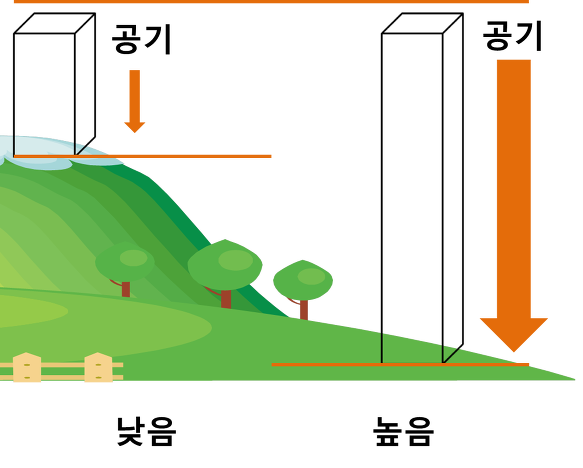
\includegraphics[width=0.95\linewidth]{21observing/images/airPressuire}
	\end{minipage}
	\begin{minipage}{.45\textwidth}
	\centering
	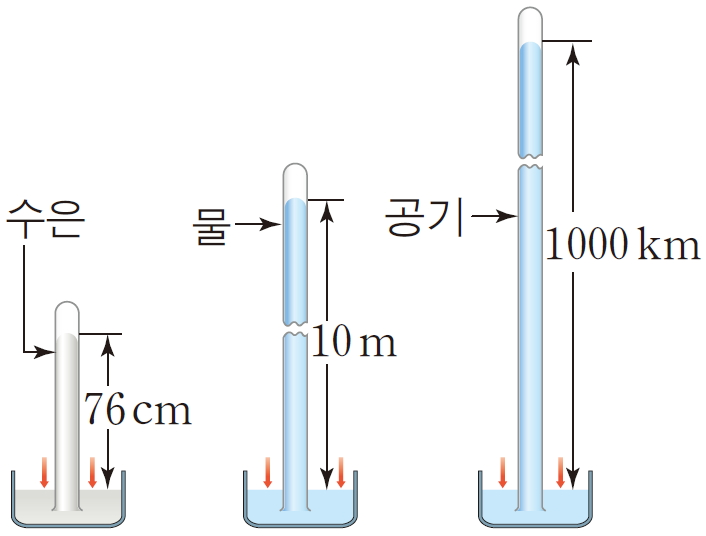
\includegraphics[width=0.95\linewidth]{21observing/images/4_14_a_7}
	\end{minipage}
	\caption{높이에 따른 기압 변화와 1기압의 크기}
	\label{fig:414a7}
\end{figure}

압력의 기본 단위는 파스칼 (Pa) 혹은 ($\rm {N~m^{-2}})$이지만 기압의 단위로는 앞에 100을 의미하는 헥토 (hecto)를 붙여서 헥토파스칼(hPa)을 사용한다. 기존에 많이 사용되었던 밀리바(mb)와 hPa은 같은 값이며, 몇몇 기압계들은 그 눈금 단위를 밀리바나 수은주 높이(mmHg)로 표시할 수 있는데, 표준 대기 상태에서 기압이 1013.250 일 때 수은주는 760 mmHg 의 높이를 가지게 되므로 기압의 단위는 다음과 같이 변환할 수 있다.
	
1 hPa = 0.750062(mmHg)

기압은 현재의 대기의 상태를 분석을 통해서 예측으로 이어지는 일련의 기상 업무에서 가장 기본적인 요소이므로 반드시 관측이 이루어져야 하므로, 대기 관측에서 사용되는 수은 기압계는 표준 기온 0$\rm ^{\circ}C$, 중력 가속도 9.80665($\rm m~s^{-2}$) 에서 다음과 같은 요구 조건들을 만족하여야 한다.

\begin{itemize}
	\item 관측 범위 : 500 - 1080
	\item 불확실성(오차) : 0.1 이하
	\item 보고 단위 : 0.1
	\item 관측 센서 지속 시간 : 20초
	\item 자료 표출 주기 : 1분 이하
\end{itemize}

\subsection{기온}\index{기온}

대기관측에 있어서 온도는 다양한 매체를 상대로 측정한다. 가장 일반적인 측정 변수는 다양한 고도에 대한 기온이고, 다른 것들로는 지표면, 토양, 잔디, 해수면 온도 등이다. WMO는 기온을 “태양의 직접 복사로부터 차폐된 곳의 공기 중에 노출된 온도계가 가리키는 온도”로 정의하고 있다. 비록 이 정의가 그 자체의 열역학적 물리량으로 정의되는 것은 아니지만 광범위 하게 적용되고 있다.

대기관측에서 온도 관측은 다음과 같은 대상을 상대로 실시한다.
\begin{itemize}
	\item 지표면 근처 대기
	\item 지표면
	\item 다양한 깊이의 토양
	\item 해수면과 대형 호수면
	\item 상층 대기
\end{itemize}

대기 관측에 사용되는 온도계들은 보정 범위와 계산 오차의 크기가 정해진 기준 이내에 들어있는 것을 사용해야 한다. 또한 온도계의 운영 범위는 국지적인 기후 범위에 맞추어 선택되어야 한다. Table \ref{table:22} \은 온도계의 허용 가능한 보정 및 오차 범위를 보여주고 있다.

\begin{table}[h]
	\centering
	\caption{온도계의 허용 가능한 보정 및 오차 범위}
\begin{tabular}{c|c|c|c}
	\hline 
	온도계 종류 & 정규 온도계 & 최고 기온 온도계 & 최저 기온 온도계 \\ 	\hline 
	온도 척도 범위 & -30 - 45 & -30 - 50 & -40-40 \\ 	\hline 
	보정 범위 & -30 - 40 & -25 - 40 & -30 - 30 \\ \hline 
	최대 허용 오차 & < 0.2K  & 0.2K & 0.3K  \\ 	\hline 
\end{tabular} 
	\label{table:22}
\end{table}

온도계를 읽을 때 시간 상수를 너무 길게 잡으면 짧은 온도 변화 경향을 평활화 시켜버릴 수 있고, 너무 짧게 잡으면 큰 범위의 온도 변화 경향을 보는데 불리하다. 보통의 경우 온도계의 감응 시간은 20초를 기준으로 삼는다. 

온도는 지표면 상태, 식생, 건물의 존재, 백엽상의 모양 등과 같은 주변 환경의 변화에 매우 민감하게 변화하기 때문에 온도 자료를 저장할 때는 관측 환경의 변화에 관해서도 동시에 기록하는 것이 좋다. 이렇게 어떤 기상 변수에 대한 정보를 기록하는 것을 ‘자료에 대한 자료(Metadata)’라고 부른다.

\subsection{습도}\index{습도}

WMO는 대기 중의 습도를 나타내는 정의들을 제시하고 있는데, 대기 과학에서 자주 사용하는 대기 중의 습기의 척도를 나타내는 변수들은 다양하다.

\begin{itemize}
	\item 혼합비(r) : 건조 공기 질량 대 수증기 질량의 비
	\item 비습(q) : 습윤 공기 질량 대 수증기 질량의 비
	\item 노점 온도($\rm T_d$) : 주어진 기압에서 포화 혼합비와 주어진 혼합비가 같아 습윤 공기가 포화되는 온도
	\item 상대습도 (U) : 같은 온도와 기압에서 물의 포화 수증기압에 대한 관측된 수증기압의 비를 \%로 나타낸 것
	\item 수증기압($\rm e^{\prime}$) : 공기 중의 수증기의 분압
	\item 포화 수증기압($\rm e_w^{\prime}$ 와 $\rm e_i^{\prime}$) : 물과 얼음의 표면과 공기가 평형을 이루는 상태의 수증기압
\end{itemize}
대기 중의 수증기와 관련된 변수들의 단위와 척도는 다음과 같이 정리할 수 있다.
\begin{itemize}
	\item 혼합비(r)와 비습(q) : kg/kg
	\item 공기의 수증기압 ($\rm e ^{\prime}$, $\rm e_w^{\prime}$, $\rm e_i^{\prime}$) : hPa
	\item 온도(T), 습구 온도($\rm T_w$), 노점 온도($\rm T_d$), 빙점 온도($\rm T_f$) : K, ($\rm ^{\circ}C$) 
	\item 상대 습도(U) : \%
\end{itemize}

지표면 부근의 습도 관측은 기상 분석 및 예보, 기후 연구, 수문학, 농업 기상학, 항공 기상, 환경 연구 등을 위해서 반드시 필요한 요소이다. 대기 속에서의 물의 상변화는 기상 현상의 발생에서 소멸까지 매우 중요한 변수가 될 수 있다. 
습도 관측 시 고려해야 할 관측 범위, 해상도, 정확도는 아래 표 \ref{table:33} \과 같다.

\begin{table}[h]
	\centering
	\caption{지상 습도 관측 요구 조건들}
\begin{tabular}{c|c|c|c}
	\hline 
	요구 조건 & 습구 온도 & 상대 습도 & 노점 온도 \\ 
	\hline 
	관측 범위 & -10$\rm ^{\circ}C$ - 35$\rm ^{\circ}C$ & 5 \% - 100 \% & -60 - 35$\rm ^{\circ}C$   \\ 
	\hline 
	정확도(불확실성) & 0.1 - 0.2 K & 1 - 5 \% & 0.1 - 0.5K \\ 
	\hline 
	허용 오차 & 0.2 K & 3 - 5 \% & 0.5 K \\ 
	\hline 
	보고 해상도 & 0.1 K & 1 \% & 0.1 K \\ 
	\hline 
	평균 시간 & 60초 & 60초 & 60초 \\ 
	\hline 
\end{tabular} 
	\label{table:33}
\end{table}


\subsection{바람}\index{바람}

바람은 공기의 수직적 수평적 흐름으로 3차원 벡터 값으로 표현할 수 있지만 대기 오염이나 항공기 이착륙 등과 같은 특수한 상황을 제외하고 일반적으로는 풍속은 이차원 벡터 즉 수평 방향과 속도 성분만을 가지는 것으로 정의한다.
바람에 대한 정보는 순간적인 정보가 아닌 평균된 바람장과 순간풍 정보를 동시에 포함하고 있어야 하기 때문에 바람 관측 장비는 관측 센서뿐만 아니라 데이터 처리와 기록 시스템이 포함되어 있어야 한다. 바람 관측자료를 처리할 때에는 평균, 표준편차 계산 등에서 오류가 발생하지 않도록 해야 하고 순간 최대풍에 대한 정보가 평활화되어 없어지지 않도록 유의해야 한다. 

순간 최대풍은 일정한 시간 간격 동안 관측된 최대 풍속을 의미한다. 1시간 단위 관측에서 순간 최대풍은 1시간 동안 나타났던 최대 풍속을 의미한다. 순간풍 기간은 순간 최대풍이 관측되었던 기간을 의미하는데, 느리게 반응하는 관측장비의 경우에는 실제 순간풍을 실제 보다 낮게 나타낼 수 있고 너무 빠르게 반응하는 장비는 짧은 시간에 파동 형태의 풍속 변동을 보여 탁월풍을 한 눈에 알아보기 힘들게 할 수도 있다.

평균풍은 10분에서 60분 평균된 수평 바람 정보를 말하는데 보통 기상예보에 활용하는 경우에는 10분 평균 바람 정보를 이용하고 있다.풍속의 정확도는 평균 풍속 5 m/s 이하에서는 0.5 m/s, 평균 풍속 5 m/s 이상에서는 그 풍속의 10\% 미만이면 충분하고 풍향은 5$\rm ^{\circ}$ 범위 내에서 정확도를 가지고 있어야 하는데, 최근 관측장비들은 이러한 요구 조건들을 충분히 만족할 만큼 정확도가 뛰어나다.

\begin{figure}[h!]
	\centering
	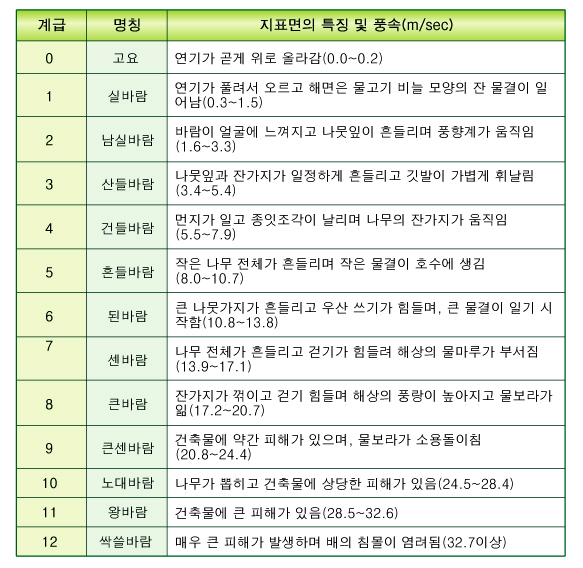
\includegraphics[width=0.9\linewidth]{21observing/images/11120_1_2}
	\caption{보퍼트 풍력계급}
	\label{fig:1112012}
\end{figure}


\subsection{구름}\index{구름}

구름은 관측 지점에서 인지가 가능한 아주 작은 수적, 얼음 알갱이 혹은 두 가지의 혼합물들의 집합체로 지표면 상공에 떠 있는 것을 의미한다. 구름 속 수적 입자는 반지름이 200 미만으로 반지름이 이것보다 커지면 그 수적은 이슬비나 비로 추정한다. 아주 특별하고 드물게 나타나는 진주모운이나 야광운, 성층권 하부에서 가끔 발생하는 권운의 경우를 제외하고는 거의
대부분의 구름의 발생은 대류권 내로 제한된다. 
%구름은 대류활동, 지형에 의한 강제상승, 저기압, 전선과 같은 대규모 연직 운동 등과 같은 공기의 연직 운동의 결과로 만들어진다. 구름이 형성에는 적절한 기온감률과 대기 중 습기, 하층 난류 등과 같은 작은 요인들도 작용한다. 
%기온이 0℃ 이하인 상운형을 관측하고 지표면으로부터의 운저고도를 추정하거나 측정하는 것은 여러 가지 목적에서 중요한 요소이다. 특히 항공기상과 응용기상 분야에서 그 중요성은 무시할 수 없다. 기본적으로 관측자와 예보관들은 구름의 형태와 특성에 대해서 충분히 이해하고 있어야 한다.
%태에서도 구름 입자들은 전부 수적으로 이루어질 수 있는데 보통 층운의 경우에는 -0℃까지 대류운의 경우에는 -5℃까지 과냉각 수적의 형태로 존재한다. 이 온도 기준보다 낮아지면 수적들이 얼음 알갱이로 변하고 구름 속에는 과냉각 수적과 얼음이 혼합되어 존재하게 된다.

\subsubsection{운량}
가장 효과적이고 많이 사용되는 운량 관측은 관측자의 목측에 의한 것이다. 관측 장비를 사용하는 방법은 여전히 개발 중이지만 알고리즘을 이용하여 하층운에 대한 운량을 추정하는 정도에 그치고 있다. 운량은 식별되는 층의 운량과 전체 층의 총운량이 동시에 보고되어야 한다. 총운량은 보이는 모든 구름들을 모았을 때 전체 하늘을 가리는 정도를 옥타로 표현한 것이다. 층
별 부분 운량은 동일한 구름의 형태나 구름의 층이 하늘을 가리는 정도를 의미하는데 부분 운량을 모두 합치면 총운량이나 8옥타를 넘을 수도 있다.

WMO가 정한 운량에 대한 코드는 다음과 같다.

\begin{figure}[h]
	\centering
	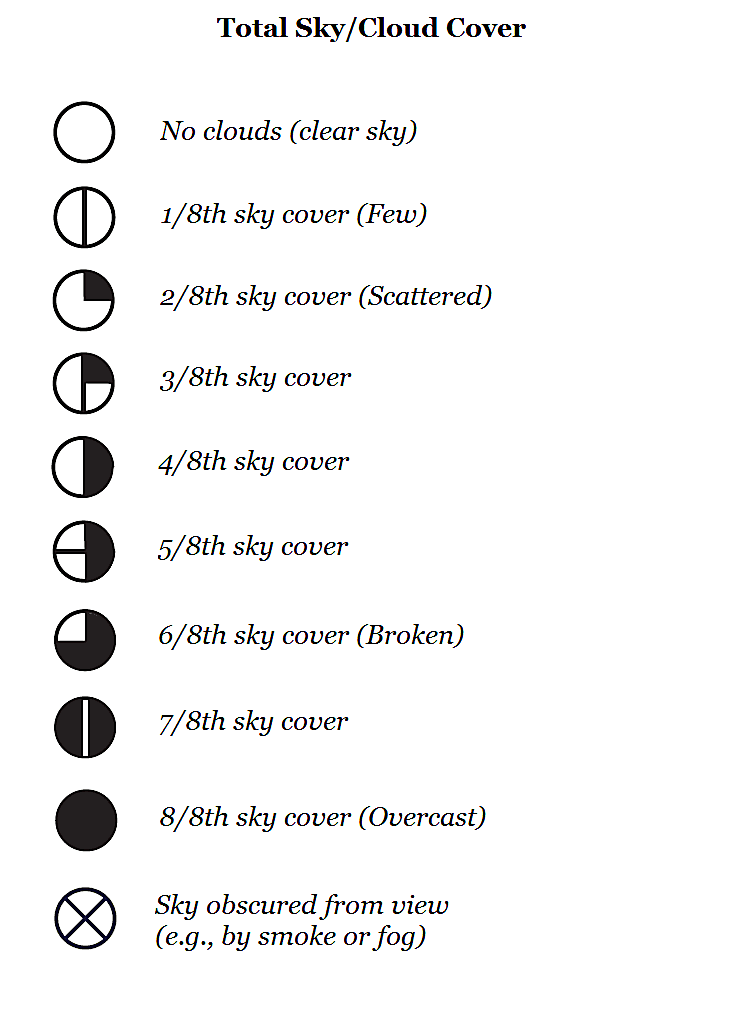
\includegraphics[width=0.4\linewidth]{21observing/images/sky-cover_key-58b740215f9b5880804caa18}
	\caption{운량}
	\label{fig:okta}
\end{figure}

\subsubsection{운저 고도}
구름의 운저 고도는 항공기상을 비롯한 기상업무에 매우 중요한 요소이기 때문에 대부분 관측장비를 사용해서 관측하지만 여전히 관측자에 의한 목측에 의존하는 경우도 많다. 구름 관측을 보고할 때는 관측 장비의 정확도에 대한 정보가 같이 포함되어야 하는데 특히 항공 기상에서 운저 고도는 항공기 운항 조건을 결정하는 요소이므로 매우 높은 정밀도를 요구한다.

\subsubsection{운형}
운량과 마찬가지로 현재까지 운형을 파악할 수 있는 유일한 수단은 관측자의 목측 밖에 없다. 관측자들은 운형 사진과 운형 도감을 활용해서 다양한 형태의 운형에 대해서 인지하고 있어야 한다.

\begin{figure}[]
	\centering
	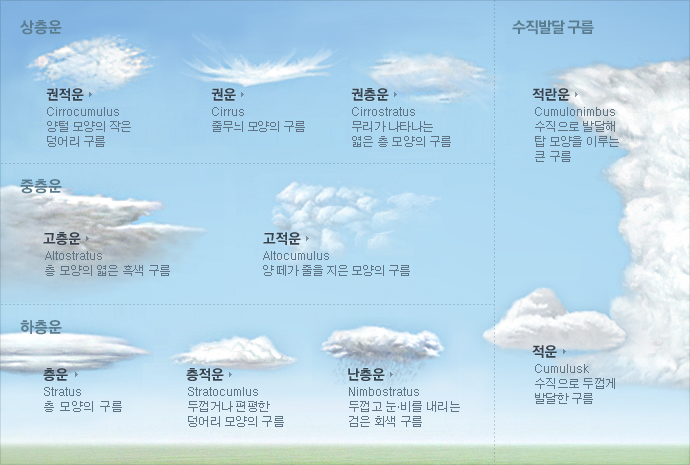
\includegraphics[width=0.95\linewidth]{21observing/images/20}
	\caption{구름의 분류}
	\label{fig:20}
\end{figure}

\subsection{강수}\index{강수}

강수량계(혹은 우량계)는 가장 많이 사용되는 강수 관측 장비이다. 일반적으로 우량계는 상부에 강수를 모으는 용기가 있고, 아래에 모인 강수량을 측정할 수 있는 원통 형태의 실린더를 가지는데 전체적인 모양은 깔때기 형태이다.

강수 측정은 설치 장소와 바람에 따라 큰 차이를 보일 수 있는데 강수 관측은 우량계의 설치 위치에 따라 민감한 차이를 보이기 때문에 강수 관측자료에는 우량계 주변의 특이한 장애물의 수직각, 우량계의 구성, 우량계 입구의 높이, 바람 관측장비의 높이 등과 같은 관측 환경에 대한 부가적인 정보가 포함되어야 한다. 한 지점에서의 다른 형태의 우량계 사용, 우량계 위치나 높이의 변화 등은 강수 관측자료의 시간적 불균일성을 가져올 수 있고, 지점 별로 다른 형태의 우량계 사용, 설치 특성의 차이는 공간적인 불균일성을 가져와 강수 관측의 체계 오차를 만들어 낼 수 있는데 가장 큰 요인은 바람에 의해서 강수 입자가 수평적으로 날리는 현상이다.

\newpage

\section{데이터 처리하기}\index{데이터 처리하기}

\subsection{기온의 일변화}\index{기온의 일변화}
1. 주어진 자료 중에서 봄, 여름, 가을, 겨울 각각에 해당하는 날을 하루씩 선정하여 아래와 같은 모양의 차트를 완성해 보자.

\begin{figure}[h!]
	\begin{tikzpicture}
	\begin{axis} [
	width=1.00\textwidth,%
	height = 9cm,%
	xtick = data,%
	symbolic x coords={00, 01, 02, 03, 04, 05, 06, 07, 08, 09, 10, 11, 12, 13, 14, 15, 16, 17, 18, 19, 20, 21, 22, 23},%
	ylabel= {온도 ($\rm ^{\circ}C$)},%
	ymin=-20,ystep=5,ymax=50.0,%
	scaled y ticks = false,%
	%ymajorgrids = true,
	legend style={at={(0.02,10)}},legend pos=north west]%
	\addplot [style={red,fill=red,mark=x}] table [x=Month, y=Temperature] {./21observing/data/daily.csv}; \addlegendentry {Temperature}%
	\end{axis}
	
	\begin{axis} [
	width=1.00\textwidth,height = 9cm,%
	axis y line*=right,%
	xtick=data,%
	symbolic x coords={00, 01, 02, 03, 04, 05, 06, 07, 08, 09, 10, 11, 12, 13, 14, 15, 16, 17, 18, 19, 20, 21, 22, 23},%
	ylabel= {습도 ($\rm \%$)},%
	ymin=0,ystep=10,ymax=100.0,%
	scaled y ticks=false,%
	legend style={at={(0.02,0.02)}},legend pos=north east]
	\addplot [style={blue,fill=blue,mark=o}] table [x=Month, y=Humidity] {./21observing/data/daily.csv}; \addlegendentry {Humidity}%
	\end{axis}
	\end{tikzpicture}
	\scriptsize\caption{하루 동안 기온과 습도의 5분 평균 값의 변동}
	\label{fig:diff_2003}
\end{figure}

2. 주어진 자료 중에서 봄, 여름, 가을, 겨울 각각에 해당하는 날을 하루씩 선정하여 아래와 같은 모양의 차트를 완성해 보자.
\begin{figure}[h!]
	\begin{tikzpicture}
	\begin{axis} [
	width=1.00\textwidth,%
	height = 9cm,%
	xtick = data,%
	symbolic x coords={00, 01, 02, 03, 04, 05, 06, 07, 08, 09, 10, 11, 12, 13, 14, 15, 16, 17, 18, 19, 20, 21, 22, 23},%
	ylabel= {온도 ($\rm ^{\circ}C$)},%
	ymin=-20,ystep=5,ymax=50.0,%
	scaled y ticks = false,%
	%ymajorgrids = true,
	legend style={at={(0.02,10)}},legend pos=north west]%
	\addplot [style={red,fill=red,mark=x}] table [x=Month, y=Temperature] {./21observing/data/daily.csv}; \addlegendentry {Temperature}%
	\end{axis}
	
	\begin{axis} [
	width=1.00\textwidth,height = 9cm,%
	axis y line*=right,%
	xtick=data,%
	symbolic x coords={00, 01, 02, 03, 04, 05, 06, 07, 08, 09, 10, 11, 12, 13, 14, 15, 16, 17, 18, 19, 20, 21, 22, 23},%
	ylabel= {습도 ($\rm \%$)},%
	ymin=0,ystep=10,ymax=100.0,%
	scaled y ticks=false,%
	legend style={at={(0.02,0.02)}},legend pos=north east]
	\addplot [style={blue,fill=blue,mark=o}] table [x=Month, y=Humidity] {./21observing/data/daily.csv}; \addlegendentry {Humidity}%
	\end{axis}
	\end{tikzpicture}
	\scriptsize\caption{하루 동안 기온과 습도의 1시간 평균 값의 변동}
	\label{fig:diff_2003}
\end{figure}

\newpage
\subsection{기온의 년변화}\index{기온의 년변화}
1. 주어진 자료로 1년 동안 매일 매일의 일평균 값을 구한 후 아래와 모양의 차트를 완성해 보자.

\pgfdeclarelayer{foreground}
\pgfsetlayers{foreground,main}

\begin{figure}[h!]
	\begin{tikzpicture}
	\begin{axis} [
	width=1.00\textwidth,%
	height = 9cm,%
	xtick = data,%
	symbolic x coords={Jan, Feb, Mar, Apr, May, Jun, Jul, Aug, Sep, Oct, Nov, Dec},%
	ylabel= {온도 ($\rm ^{\circ}C$)},%
	ymin=-20,ystep=5,ymax=50.0,%
	scaled y ticks = false,%
	%ymajorgrids = true,
	legend style={at={(0.02,10)}},legend pos=north west]%
	\addplot [style={red,fill=red,mark=x}] table [x=Month, y=Temperature] {./21observing/data/monthly.csv}; \addlegendentry {Temperature}%
	\end{axis}
	
	\begin{axis} [
	width=1.00\textwidth,height = 9cm,%
	axis y line*=right,%
	xtick=data,%
	symbolic x coords={Jan, Feb, Mar, Apr, May, Jun, Jul, Aug, Sep, Oct, Nov, Dec},%
	ylabel= {습도 ($\rm \%$)},%
	ymin=0,ystep=10,ymax=100.0,%
	scaled y ticks=false,%
	legend style={at={(0.02,0.02)}},legend pos=north east]
	\addplot [style={blue,fill=blue,mark=o}] table [x=Month, y=Humidity] {./21observing/data/monthly.csv}; \addlegendentry {Humidity}%
	\end{axis}
	\end{tikzpicture}
	\scriptsize\caption{연간 기온과 습도의 일평균 값의 변동}
	\label{fig:diff_2003}
\end{figure}

2. 주어진 자료로 1년 동안 매일 매일의 월평균 값을 구한 후 아래와 모양의 차트를 완성해 보자.
\pgfdeclarelayer{foreground}
\pgfsetlayers{foreground,main}

\begin{figure}[h!]
	\begin{tikzpicture}
	\begin{axis} [
	width=1.00\textwidth,%
	height = 9cm,%
	xtick = data,%
	symbolic x coords={Jan, Feb, Mar, Apr, May, Jun, Jul, Aug, Sep, Oct, Nov, Dec},%
	ylabel= {온도 ($\rm ^{\circ}C$)},%
	ymin=-20,ystep=5,ymax=50.0,%
	scaled y ticks = false,%
	%ymajorgrids = true,
	legend style={at={(0.02,10)}},legend pos=north west]%
	\addplot [style={red,fill=red,mark=x}] table [x=Month, y=Temperature] {./21observing/data/monthly.csv}; \addlegendentry {Temperature}%
	\end{axis}
	
	\begin{axis} [
	width=1.00\textwidth,height = 9cm,%
	axis y line*=right,%
	xtick=data,%
	symbolic x coords={Jan, Feb, Mar, Apr, May, Jun, Jul, Aug, Sep, Oct, Nov, Dec},%
	ylabel= {습도 ($\rm \%$)},%
	ymin=0,ystep=10,ymax=100.0,%
	scaled y ticks=false,%
	legend style={at={(0.02,0.02)}},legend pos=north east]
	\addplot [style={blue,fill=blue,mark=o}] table [x=Month, y=Humidity] {./21observing/data/monthly.csv}; \addlegendentry {Humidity}%
	\end{axis}
	\end{tikzpicture}
	\scriptsize\caption{연간 기온과 습도의 월평균 값의 변동}
	\label{fig:diff_2003}
\end{figure}

